\section{The straight lines}

It is of course essential to draw straight lines, but before this can be done, it is necessary to be able to define certain particular lines such as mediators, bisectors, parallels or even perpendiculars. The principle is to determine two points on the straight line. 


\subsection{Definition of straight lines}

\begin{NewMacroBox}{tkzDefLine}{\oarg{local options}\parg{pt1,pt2} or \parg{pt1,pt2,pt3}}%
The argument is a list of two or three points. Depending on the case, the macro defines one or two points necessary to obtain the line sought. Either the macro \tkzcname{tkzGetPoint} or the macro \tkzcname{tkzGetPoints} must be used.

\medskip
\begin{tabular}{lll}%
\toprule
arguments           & example & explication                         \\
\midrule
\TAline{\parg{pt1,pt2}}{\parg{A,B}} {[mediator](A,B)}
\TAline{\parg{pt1,pt2,pt3}}{\parg{A,B,C}} {[bisector](B,A,C)}
\end{tabular}

\medskip
\begin{tabular}{lll}%
\toprule
options             & default & definition                         \\ 
\TOline{mediator}{}{two points are defined} 
\TOline{perpendicular=through\dots}{mediator}{perpendicular to a straight line passing through a point} 
\TOline{orthogonal=through\dots}{mediator}{see above }
\TOline{parallel=through\dots}{mediator}{parallel to a straight line passing through a point}
\TOline{bisector}{mediator}{bisector of an angle defined by three points}
\TOline{bisector out}{mediator}{Exterior Angle Bisector}
\TOline{K}{1}{coefficient for the perpendicular line}
\TOline{normed}{false}{normalizes the created segment}
\end{tabular}
\end{NewMacroBox}  

\subsubsection{Example with \tkzname{mediator}}  
\begin{tkzexample}[latex=5 cm,small]
\begin{tikzpicture}[rotate=25]
 \tkzDefPoints{-2/0/A,1/2/B}
 \tkzDefLine[mediator](A,B)          \tkzGetPoints{C}{D}
 \tkzDefPointWith[linear,K=.75](C,D) \tkzGetPoint{D}
 \tkzDefMidPoint(A,B)                \tkzGetPoint{I}
 \tkzFillPolygon[color=orange!30](A,C,B,D)
 \tkzDrawSegments(A,B C,D)
 \tkzMarkRightAngle(B,I,C) 
 \tkzDrawSegments(D,B D,A)
 \tkzDrawSegments(C,B C,A)
\end{tikzpicture}
\end{tkzexample}  

\subsubsection{Example with \tkzname{bisector} and \tkzname{normed}} 
\begin{tkzexample}[latex=7 cm,small] 
\begin{tikzpicture}[rotate=25,scale=.75]
 \tkzDefPoints{0/0/C, 2/-3/A, 4/0/B}
 \tkzDefLine[bisector,normed](B,A,C) \tkzGetPoint{a}
 \tkzDrawLines[add= 0 and .5](A,B A,C)
 \tkzShowLine[bisector,gap=4,size=2,color=red](B,A,C)
 \tkzDrawLines[blue!50,dashed,add= 0 and 3](A,a)
\end{tikzpicture}
\end{tkzexample} 

\subsubsection{Example with \tkzname{orthogonal} and \tkzname{parallel}}    
\begin{tkzexample}[latex=5 cm,small]
\begin{tikzpicture}
   \tkzDefPoints{-1.5/-0.25/A,1/-0.75/B,-0.7/1/C}
   \tkzDrawLine(A,B)
   \tkzLabelLine[pos=1.25,below left](A,B){$(d_1)$}
   \tkzDrawPoints(A,B,C)
   \tkzDefLine[orthogonal=through C](B,A) \tkzGetPoint{c}
   \tkzDrawLine(C,c) 
   \tkzLabelLine[pos=1.25,left](C,c){$(\delta)$}
   \tkzInterLL(A,B)(C,c) \tkzGetPoint{I}
   \tkzMarkRightAngle(C,I,B) 
   \tkzDefLine[parallel=through C](A,B) \tkzGetPoint{c'}
   \tkzDrawLine(C,c') 
   \tkzLabelLine[pos=1.25,below left](C,c'){$(d_2)$}
   \tkzMarkRightAngle(I,C,c')   
\end{tikzpicture}
\end{tkzexample}

\subsubsection{An envelope}
Based on a figure from O. Reboux with pst-eucl by D Rodriguez.

\begin{tkzexample}[vbox,small]
\begin{tikzpicture}[scale=.75]
 \tkzInit[xmin=-6,ymin=-4,xmax=6,ymax=6] % necessary
 \tkzClip
 \tkzDefPoint(0,0){O} 
 \tkzDefPoint(132:4){A}
 \tkzDefPoint(5,0){B}
 \foreach \ang in {5,10,...,360}{%
  \tkzDefPoint(\ang:5){M}
  \tkzDefLine[mediator](A,M)
  \tkzDrawLine[color=magenta,add= 3 and 3](tkzFirstPointResult,tkzSecondPointResult)}
\end{tikzpicture}
\end{tkzexample}

\subsubsection{A parabola}
Based on a figure from O. Reboux with pst-eucl by D Rodriguez.
It is not necessary to name the two points that define the mediator.

\begin{tkzexample}[vbox,small]
\begin{tikzpicture}[scale=.75]
 \tkzInit[xmin=-6,ymin=-4,xmax=6,ymax=6] 
 \tkzClip
 \tkzDefPoint(0,0){O} 
 \tkzDefPoint(132:5){A}
 \tkzDefPoint(4,0){B}
 \foreach \ang in {5,10,...,360}{%
  \tkzDefPoint(\ang:4){M}
  \tkzDefLine[mediator](A,M) 
  \tkzDrawLine[color=magenta,add= 3 and 3](tkzFirstPointResult,tkzSecondPointResult)}
\end{tikzpicture}
\end{tkzexample}

%<---------------------------------------------------------------------------->
\subsection{Specific lines:  Tangent to a circle}
Two constructions are proposed. The first one is the construction of a tangent to a circle at a given point of this circle and the second one is the construction of a tangent to a circle passing through a given point outside a disc. 

\begin{NewMacroBox}{tkzDefTangent}{\oarg{local options}\parg{pt1,pt2} or \parg{pt1,dim}}%
The parameter in brackets is the center of the circle or the center of the circle and a point on the circle or the center and the radius. This macro replaces the old one: \tkzcname{tkzTangent}.

\medskip
\begin{tabular}{lll}%
\toprule
arguments           & example & explication                         \\
\midrule
\TAline{\parg{pt1,pt2 or \parg{pt1,dim}} }{\parg{A,B} or \parg{A,2cm}} {$[AB]$ is radius $A$ is the center}
\bottomrule
\end{tabular} 

\medskip
\begin{tabular}{lll}%
options             & default & definition                         \\ 
\midrule
\TOline{at=pt}{at}{tangent to a point on the circle} 
\TOline{from=pt} {at}{tangent to a circle passing through a point}
\TOline{from with R=pt} {at}{idem, but the circle is defined by center = radius}  
\bottomrule
\end{tabular}

The tangent is not drawn. A second point of the tangent is given by \tkzname{tkzPointResult}.
\end{NewMacroBox}

\subsubsection{Example of a tangent passing through a point on the circle } 
\begin{tkzexample}[latex=7cm,small]
\begin{tikzpicture}[scale=.75]
  \tkzDefPoint(0,0){O}
  \tkzDefPoint(6,6){E}
  \tkzDefRandPointOn[circle=center O radius 3cm]
  \tkzGetPoint{A}
  \tkzDrawSegment(O,A)
  \tkzDrawCircle(O,A)
  \tkzDefTangent[at=A](O)
  \tkzGetPoint{h}
  \tkzDrawLine[add = 4 and 3](A,h)
  \tkzMarkRightAngle[fill=red!30](O,A,h)
\end{tikzpicture}
\end{tkzexample}

\subsubsection{Example of tangents passing through an external point } 
\begin{tkzexample}[latex=7cm,small]
\begin{tikzpicture}[scale=.8] 
  \tkzDefPoint(3,3){c}
  \tkzDefPoint(6,3){a0}  
  \tkzRadius=1 cm 
  \tkzDrawCircle[R](c,\tkzRadius) 
  \foreach \an in {0,10,...,350}{
     \tkzDefPointBy[rotation=center c angle \an](a0)  
     \tkzGetPoint{a}  
     \tkzDefTangent[from with R = a](c,\tkzRadius)  
     \tkzGetPoints{e}{f} 
     \tkzDrawLines[color=magenta](a,f a,e) 
      \tkzDrawSegments(c,e c,f)
      }%
\end{tikzpicture} 
\end{tkzexample}

\subsubsection{Example of Andrew Mertz}
\begin{tkzexample}[latex=6cm,small]
 \begin{tikzpicture}[scale=.5] 
 \tkzDefPoint(100:8){A}\tkzDefPoint(50:8){B}  
 \tkzDefPoint(0,0){C} \tkzDefPoint(0,4){R} 
 \tkzDrawCircle(C,R)
 \tkzDefTangent[from = A](C,R)  \tkzGetPoints{D}{E}
 \tkzDefTangent[from = B](C,R)  \tkzGetPoints{F}{G}
 \tkzDrawSector[fill=blue!80!black,opacity=0.5](A,D)(E)
 \tkzFillSector[color=red!80!black,opacity=0.5](B,F)(G)
 \tkzInterCC(A,D)(B,F) \tkzGetSecondPoint{I}
 \tkzDrawPoint[color=black](I)
 \end{tikzpicture}
\end{tkzexample}
\url{http://www.texample.net/tikz/examples/}  

\subsubsection{Drawing a tangent option \tkzimp{from with R} and \tkzimp{at}}
\begin{tkzexample}[latex=7cm,small]
  \begin{tikzpicture}[scale=.5] 
  \tkzDefPoint(0,0){O}
  \tkzDefRandPointOn[circle=center O radius 4cm]
  \tkzGetPoint{A}
  \tkzDefTangent[at=A](O)
  \tkzGetPoint{h}
  \tkzDrawSegments(O,A) 
  \tkzDrawCircle(O,A) 
  \tkzDrawLine[add = 1 and 1](A,h)
  \tkzMarkRightAngle[fill=red!30](O,A,h)
  \end{tikzpicture}
\end{tkzexample}

\subsubsection{Drawing a tangent option \tkzimp{from}}
\begin{tkzexample}[latex=5cm,small]
\begin{tikzpicture}[scale=.5] 
 \tkzDefPoint(0,0){B} 
 \tkzDefPoint(0,8){A} 
 \tkzDefSquare(A,B)
 \tkzGetPoints{C}{D}
 \tkzDrawSquare(A,B)
 \tkzClipPolygon(A,B,C,D)
 \tkzDefPoint(4,8){F}
 \tkzDefPoint(4,0){E}
 \tkzDefPoint(4,4){Q}
 \tkzFillPolygon[color = green](A,B,C,D)
 \tkzDrawCircle[fill = orange](B,A)
 \tkzDrawCircle[fill = purple](E,B)  
 \tkzDefTangent[from=B](F,A)
 \tkzInterLL(F,tkzFirstPointResult)(C,D)
 \tkzInterLL(A,tkzPointResult)(F,E) 
 \tkzDrawCircle[fill = yellow](tkzPointResult,Q)  
 \tkzDefPointBy[projection= onto B--A](tkzPointResult)
 \tkzDrawCircle[fill = blue!50!black](tkzPointResult,A)
\end{tikzpicture}
\end{tkzexample}


\section{Drawing, naming the lines}
The following macros are simply used to draw, name lines.
\subsection{Draw a straight line}
To draw a normal straight line, just give a couple of points. You can  use the \tkzname{add} option to extend the line (This option is due to \tkzimp{Mark Wibrow}, see the code below). 

\begin{tkzltxexample}[]
  \tikzset{%
    add/.style args={#1 and #2}{
        to path={%
 ($(\tikztostart)!-#1!(\tikztotarget)$)--($(\tikztotarget)!-#2!(\tikztostart)$)%
  \tikztonodes}}}
\end{tkzltxexample}

In the special case of lines defined in a triangle, the number of arguments is a list of three points (the vertices of the triangle). The second point is where the line will come from. The first and last points determine the target segment. The old method has therefore been slightly modified. So for \tkzcname{tkzDrawMedian}, instead of $(A,B)(C)$ you have to write $(B,C,A)$ where $C$ is the point that will be linked to the middle of the segment $[A,B]$.

\begin{NewMacroBox}{tkzDrawLine}{\oarg{local options}\parg{pt1,pt2} or \parg{pt1,pt2,pt3}}%
The arguments are a list of two points or three points.

\begin{tabular}{lll}%
\toprule
options             & default & definition                         \\ 
\midrule
\TOline{median}{none}{[median](A,B,C) median from $B$}
\TOline{altitude}{none}{[altitude](C,A,B) altitude from $A$} 
\TOline{bisector}{none}{[bisector](B,C,A) bisector from $C$}
\TOline{none}{none}{draw the straight line $(AB)$} 
\TOline{add= nb1 and nb2}{.2 and .2}{extends the segment} 
 \bottomrule
\end{tabular}

\tkzname{add} defines the length of the line passing through the points pt1 and pt2. Both numbers are percentages. The styles of \TIKZ\ are accessible for plots.
\end{NewMacroBox}

\subsubsection{Examples  with \tkzname{add}}
\begin{tkzexample}[latex=5cm,small]
\begin{tikzpicture}
 \tkzInit[xmin=-2,xmax=3,ymin=-2.25,ymax=2.25]
 \tkzClip[space=.25]
 \tkzDefPoint(0,0){A} \tkzDefPoint(2,0.5){B}
 \tkzDefPoint(0,-1){C}\tkzDefPoint(2,-0.5){D} 
 \tkzDefPoint(0,1){E} \tkzDefPoint(2,1.5){F} 
 \tkzDefPoint(0,-2){G} \tkzDefPoint(2,-1.5){H}
 \tkzDrawLine(A,B)    \tkzDrawLine[add = 0 and .5](C,D) 
 \tkzDrawLine[add = 1 and 0](E,F)
 \tkzDrawLine[add = 0 and 0](G,H) 
 \tkzDrawPoints(A,B,C,D,E,F,G,H)    
 \tkzLabelPoints(A,B,C,D,E,F,G,H)  
\end{tikzpicture}
\end{tkzexample} 

It is possible to draw several lines, but with the same options. 
\begin{NewMacroBox}{tkzDrawLines}{\oarg{local options}\parg{pt1,pt2 pt3,pt4 ...}}% 
Arguments are a list of pairs of  points separated by spaces.  The styles of \TIKZ\ are available for the draws. 
\end{NewMacroBox}      

\subsubsection{Example with \tkzcname{tkzDrawLines}}    

\begin{tkzexample}[latex=8cm,small]
\begin{tikzpicture}
  \tkzDefPoint(0,0){A}
  \tkzDefPoint(2,0){B}
  \tkzDefPoint(1,2){C}
  \tkzDefPoint(3,2){D}   
  \tkzDrawLines(A,B C,D A,C B,D)
  \tkzLabelPoints(A,B,C,D)
\end{tikzpicture}
\end{tkzexample}

\subsubsection{Example with  the option \tkzname{add}}   
\begin{tkzexample}[latex=8cm,small]
\begin{tikzpicture}[scale=.5]
 \tkzDefPoint(0,0){O}
 \tkzDefPoint(3,1){I}
 \tkzDefPoint(1,4){J}
 \tkzDefLine[bisector](I,O,J)     
   \tkzGetPoint{i}   
 \tkzDefLine[bisector out](I,O,J) 
   \tkzGetPoint{j}
 \tkzDrawLines[add = 1 and .5,color=red](O,I O,J) 
 \tkzDrawLines[add = 1 and .5,color=blue](O,i O,j) 
\end{tikzpicture} 
\end{tkzexample}

\subsubsection{Medians in a triangle}
\begin{tkzexample}[latex=7 cm,small]
\begin{tikzpicture}[scale=1.25]
  \tkzDefPoint(0,0){A} \tkzDefPoint(4,0){B}
  \tkzDefPoint(1,3){C} \tkzDrawPolygon(A,B,C)
  \tkzSetUpLine[color=blue]
  \tkzDrawLine[median](B,C,A)
  \tkzDrawLine[median](C,A,B)
  \tkzDrawLine[median](A,B,C)
\end{tikzpicture}
\end{tkzexample}

\subsubsection{Altitudes in a triangle}
\begin{tkzexample}[latex=7 cm,small]
\begin{tikzpicture}[scale=1.25]
 \tkzDefPoint(0,0){A} \tkzDefPoint(4,0){B}
 \tkzDefPoint(1,3){C} \tkzDrawPolygon(A,B,C)
 \tkzSetUpLine[color=magenta]
 \tkzDrawLine[altitude](B,C,A)
 \tkzDrawLine[altitude](C,A,B)
 \tkzDrawLine[altitude](A,B,C)
\end{tikzpicture}
\end{tkzexample}

\subsubsection{Bisectors in a triangle}
You have to give the angles in a straight line.

\begin{tkzexample}[latex=7 cm,small]
\begin{tikzpicture}[scale=1.25]
 \tkzDefPoint(0,0){A} \tkzDefPoint(4,0){B}
 \tkzDefPoint(1,3){C} \tkzDrawPolygon(A,B,C)
 \tkzSetUpLine[color=purple]
 \tkzDrawLine[bisector](B,C,A)
 \tkzDrawLine[bisector](C,A,B)
 \tkzDrawLine[bisector](A,B,C)
\end{tikzpicture}
\end{tkzexample}

\subsection{Add labels on a straight line \tkzcname{tkzLabelLine}}% 
\begin{NewMacroBox}{tkzLabelLine}{\oarg{local options}\parg{pt1,pt2}\marg{label}}
\begin{tabular}{lll}%
arguments &  default & definition   \\ 
\midrule
\TAline{label}{}{\tkzcname{tkzLabelLine(A,B)}\{\$\tkzcname{Delta}\$\}}
\bottomrule
\end{tabular}

\begin{tabular}{lll}%
options             & default & definition   \\ 
\midrule
\TOline{pos}{.5}{\tkzname{pos} is an option for \TIKZ, but essential in this case\dots} 
\end{tabular}

As an option, and in addition to the \tkzname{pos}, you can use all styles of \TIKZ, especially the placement with \tkzname{above}, \tkzname{right}, \dots
\end{NewMacroBox}

\subsubsection{Example with \tkzcname{tkzLabelLine}}
An important option is \tkzname{pos}, it's the one that allows you to place the label along the right. The value of \tkzname{pos} can be greater than 1 or negative.

\begin{tkzexample}[latex=6cm,small]
\begin{tikzpicture}
   \tkzDefPoints{0/0/A,3/0/B,1/1/C}
   \tkzDefLine[perpendicular=through C,K=-1](A,B)
   \tkzGetPoint{c}
   \tkzDrawLines(A,B C,c)
   \tkzLabelLine[pos=1.25,blue,right](C,c){$(\delta)$} 
   \tkzLabelLine[pos=-0.25,red,left](C,c){again $(\delta)$} 
\end{tikzpicture}
\end{tkzexample}

\section{Draw, Mark segments}
There is, of course, a macro to simply draw a segment (it would be possible, as for a half line, to create a style with \tkzcname{add}).
\subsection{Draw a segment \tkzcname{tkzDrawSegment}} 
\begin{NewMacroBox}{tkzDrawSegment}{\oarg{local options}\parg{pt1,pt2}}%
The arguments are a list of two points. The styles of \TIKZ\ are available for the drawings.
 
\medskip
\begin{tabular}{lll}%
argument    & example & definition    \\
\midrule
\TAline{(pt1,pt2)}{(A,B)}{draw the segment $[A,B]$}
\bottomrule 
\end{tabular}
 
\medskip
\begin{tabular}{lll}%
options    & example & definition    \\
\midrule
\TOline{\TIKZ\ options}{}{all \TIKZ\ options are valid.}
\TOline{add}{0 and 0}{add = $kl$ and $kr$, \dots}
\TOline{\dots}{\dots}{allows the segment to be extended to the left and right. }
\TOline{dim}{no default}{dim = \{label,dim,option\}, \dots}
\TOline{\dots}{\dots}{allows you to add dimensions to a figure.}
\bottomrule 
\end{tabular}

This is of course equivalent to \tkzcname{draw (A)--(B);} 
\end{NewMacroBox}

\subsubsection{Example with point references}     

\begin{tkzexample}[latex=6cm,small]
\begin{tikzpicture}[scale=1.5]
  \tkzDefPoint(0,0){A}
  \tkzDefPoint(2,1){B}
  \tkzDrawSegment[color=red,thin](A,B)
  \tkzDrawPoints(A,B)    
  \tkzLabelPoints(A,B)  
\end{tikzpicture}
\end{tkzexample}

\subsubsection{Example of extending an segment with option \tkzname{add}} 

\begin{tkzexample}[latex=7cm,small]
  \begin{tikzpicture}
  \tkzDefPoints{0/0/A,6/0/B,0.8/4/C}
  \tkzDefTriangleCenter[euler](A,B,C) 
  \tkzGetPoint{E}
  \tkzDrawCircle[euler,red](A,B,C)
  \tkzDrawLines[add=.5 and .5](A,B A,C B,C)
  \tkzDrawPoints(A,B,C,E)
  \tkzLabelPoints(A,B,C,E)
  \end{tikzpicture}
\end{tkzexample}

\subsubsection{Example of adding dimensions with option \tkzname{dim}} 
\begin{tkzexample}[vbox,small]
\begin{tikzpicture}[scale=4]
 \pgfkeys{/pgf/number format/.cd,fixed,precision=2}
 % Define the first two points
 \tkzDefPoint(0,0){A}
 \tkzDefPoint(3,0){B}
 \tkzDefPoint(1,1){C}
 % Draw the triangle and the points
 \tkzDrawPolygon(A,B,C)
 \tkzDrawPoints(A,B,C)
 % Label the sides
 \tkzCalcLength[cm](A,B)\tkzGetLength{ABl}
 \tkzCalcLength[cm](B,C)\tkzGetLength{BCl}
 \tkzCalcLength[cm](A,C)\tkzGetLength{ACl}
 % add dim
 \tkzDrawSegment[dim={\pgfmathprintnumber\BCl,6pt,transform shape}](C,B)
 \tkzDrawSegment[dim={\pgfmathprintnumber\ACl,6pt,transform shape}](A,C)
 \tkzDrawSegment[dim={\pgfmathprintnumber\ABl,-6pt,transform shape}](A,B)
\end{tikzpicture}
\end{tkzexample}

 
\subsection{Drawing segments \tkzcname{tkzDrawSegments}} 
If the options are the same we can plot several segments with the same macro. 

\begin{NewMacroBox}{tkzDrawSegments}{\oarg{local options}\parg{pt1,pt2 pt3,pt4 ...}}%
The arguments are a two-point couple list. The styles of \TIKZ\ are available for the plots.
\end{NewMacroBox}

\begin{tkzexample}[latex=6cm,small]
\begin{tikzpicture}
  \tkzInit[xmin=-1,xmax=3,ymin=-1,ymax=2]
  \tkzClip[space=1]
  \tkzDefPoint(0,0){A}
  \tkzDefPoint(2,1){B} 
  \tkzDefPoint(3,0){C} 
  \tkzDrawSegments(A,B B,C)
  \tkzDrawPoints(A,B,C)    
  \tkzLabelPoints(A,C) 
  \tkzLabelPoints[above](B)  
\end{tikzpicture}
\end{tkzexample}

\subsubsection{Place an arrow on segment}
\begin{tkzexample}[latex=6cm,small]
\begin{tikzpicture}
  \tikzset{
    arr/.style={postaction=decorate,
    decoration={markings, 
    mark=at position .5 with {\arrow[thick]{#1}}
      }}}
  \tkzDefPoint(0,0){A}
  \tkzDefPoint(4,-4){B}
  \tkzDrawSegments[arr=stealth](A,B)
  \tkzDrawPoints(A,B) 
\end{tikzpicture}
\end{tkzexample}

\subsection{Mark a segment \tkzcname{tkzMarkSegment}}
\hypertarget{tms}{}  
  
 \begin{NewMacroBox}{tkzMarkSegment}{\oarg{local options}\parg{pt1,pt2}}% 
The macro allows you to place a mark on a segment.

\medskip
\begin{tabular}{lll}%
\toprule
options             & default & definition   \\
\midrule
\TOline{pos}{.5}{position of the mark} 
\TOline{color}{black}{color of the mark} 
\TOline{mark}{none}{choice of the mark} 
\TOline{size}{4pt}{size of the mark}
\bottomrule
\end{tabular}

Possible marks are those provided by \TIKZ, but other marks have been created based on an idea by Yves Combe.
\end{NewMacroBox} 

\subsubsection{Several marks }
\begin{tkzexample}[latex=5cm,small] 
\begin{tikzpicture}
  \tkzDefPoint(2,1){A}
  \tkzDefPoint(6,4){B}
  \tkzDrawSegment(A,B)
  \tkzMarkSegment[color=brown,size=2pt,pos=0.4, mark=z](A,B) 
  \tkzMarkSegment[color=blue,pos=0.2, mark=oo](A,B)
  \tkzMarkSegment[pos=0.8,mark=s,color=red](A,B) 
\end{tikzpicture}
\end{tkzexample}

\subsubsection{Use of \tkzname{mark}}      
\begin{tkzexample}[latex=5cm,small] 
\begin{tikzpicture}
  \tkzDefPoint(2,1){A} 
  \tkzDefPoint(6,4){B}
  \tkzDrawSegment(A,B)
  \tkzMarkSegment[color=gray,pos=0.2,mark=s|](A,B)
  \tkzMarkSegment[color=gray,pos=0.4,mark=s||](A,B)
  \tkzMarkSegment[color=brown,pos=0.6,mark=||](A,B)
  \tkzMarkSegment[color=red,pos=0.8,mark=|||](A,B)
\end{tikzpicture}
\end{tkzexample}


\subsection{Marking segments \tkzcname{tkzMarkSegments}}
\hypertarget{tmss}{} 
 
\begin{NewMacroBox}{tkzMarkSegments}{\oarg{local options}\parg{pt1,pt2 pt3,pt4 ...}}%
Arguments are a list of pairs of points separated by spaces. The styles of \TIKZ\ are available for plots.
\end{NewMacroBox} 

\subsubsection{Marks for an isosceles triangle}      
\begin{tkzexample}[latex=6cm,small]
\begin{tikzpicture}[scale=1]
 \tkzDefPoints{0/0/O,2/2/A,4/0/B,6/2/C}
 \tkzDrawSegments(O,A A,B)
 \tkzDrawPoints(O,A,B)
 \tkzDrawLine(O,B)   
 \tkzMarkSegments[mark=||,size=6pt](O,A A,B)
\end{tikzpicture}
\end{tkzexample} 

\subsection{Another marking}   
\begin{tkzexample}[latex=5cm,small] 
 \begin{tikzpicture}[scale=1]
  \tkzDefPoint(0,0){A}\tkzDefPoint(3,2){B} 
  \tkzDefPoint(4,0){C}\tkzDefPoint(2.5,1){P}
  \tkzDrawPolygon(A,B,C)
  \tkzDefEquilateral(A,P) \tkzGetPoint{P'}
  \tkzDefPointsBy[rotation=center A angle 60](P,B){P',C'}
  \tkzDrawPolygon(A,P,P')
  \tkzDrawPolySeg(P',C',A,P,B)
  \tkzDrawSegment(C,P)
  \tkzDrawPoints(A,B,C,C',P,P')
  \tkzMarkSegments[mark=s|,size=6pt,
  color=blue](A,P P,P' P',A) 
  \tkzMarkSegments[mark=||,color=orange](B,P P',C')
  \tkzLabelPoints(A,C) \tkzLabelPoints[below](P) 
  \tkzLabelPoints[above right](P',C',B) 
\end{tikzpicture} 
\end{tkzexample}  

\hypertarget{tls}{}  
\begin{NewMacroBox}{tkzLabelSegment}{\oarg{local options}\parg{pt1,pt2}\marg{label}}
This macro allows you to place a label along a segment or a line. The options are those of \TIKZ\ for example \tkzname{pos}.

\medskip
\begin{tabular}{lll}%%
argument    & example & definition    \\
\midrule
\TAline{label}{\tkzcname{tkzLabelSegment(A,B)\{$5$\}}}{label text} 
\TAline{(pt1,pt2)}{(A,B)}{label along $[AB]$} 
\bottomrule
\end{tabular}


\medskip
\begin{tabular}{lll}%
options  & default & definition    \\
\midrule
\TOline{pos}{.5}{label's position} 
\end{tabular}
\end{NewMacroBox}  

\subsubsection{Multiple labels}      
\begin{tkzexample}[latex=7 cm,small]
\begin{tikzpicture}
\tkzInit
\tkzDefPoint(0,0){A}
\tkzDefPoint(6,0){B}
\tkzDrawSegment(A,B)
\tkzLabelSegment[above,pos=.8](A,B){$a$}
\tkzLabelSegment[below,pos=.2](A,B){$4$}
\end{tikzpicture} 
\end{tkzexample}  

\subsubsection{Labels and right-angled triangle}
\begin{tkzexample}[latex=7cm,small]
\begin{tikzpicture}[rotate=-60]
\tikzset{label seg style/.append style = {%
	        color      = red,
	        }}
\tkzDefPoint(0,1){A}
\tkzDefPoint(2,4){C}
\tkzDefPointWith[orthogonal normed,K=7](C,A)
\tkzGetPoint{B}
\tkzDrawPolygon[green!60!black](A,B,C)
\tkzDrawLine[altitude,dashed,color=magenta](B,C,A)
\tkzGetPoint{P}
\tkzLabelPoint[left](A){$A$}
\tkzLabelPoint[right](B){$B$}
\tkzLabelPoint[above](C){$C$}
\tkzLabelPoint[below](P){$P$}
\tkzLabelSegment[](B,A){$c$}
\tkzLabelSegment[swap](B,C){$a$}
\tkzLabelSegment[swap](C,A){$b$}
\tkzMarkAngles[size=1cm,
     color=cyan,mark=|](C,B,A A,C,P)
\tkzMarkAngle[size=0.75cm,
     color=orange,mark=||](P,C,B)
\tkzMarkAngle[size=0.75cm,
      color=orange,mark=||](B,A,C)
\tkzMarkRightAngles[german](A,C,B B,P,C)
\end{tikzpicture} 
\end{tkzexample}

\hypertarget{tlss}{} 
 \begin{NewMacroBox}{tkzLabelSegments}{\oarg{local options}\parg{pt1,pt2 pt3,pt4 ...}}%
The arguments are a two-point couple list. The styles of \TIKZ\ are available for plotting.
\end{NewMacroBox} 
 
\subsubsection{Labels for an isosceles triangle}      
\begin{tkzexample}[latex=6cm,small]
\begin{tikzpicture}[scale=1]
 \tkzDefPoints{0/0/O,2/2/A,4/0/B,6/2/C}
 \tkzDrawSegments(O,A A,B)
 \tkzDrawPoints(O,A,B)
 \tkzDrawLine(O,B)   
 \tkzLabelSegments[color=red,above=4pt](O,A A,B){$a$}
\end{tikzpicture}
\end{tkzexample}  
\endinput